\section*{Question 1}
On sait que $\dot{\Ha}(p,q) = 0$ car $\Ha$ est invariant dans le temps.
De plus, comme
\[
  \dot{\Ha}(p,q) = \fpart{\Ha(p,q)}{p}^T\dot{p} + \fpart{\Ha(p,q)}{q}^T\dot{q}
\]
on doit avoir
\[
  \fpart{\Ha(p,q)}{p}^T\dot{p} + \fpart{\Ha(p,q)}{q}^T\dot{q} = 0.
\]

Les équations
\begin{align*}
  \dot{q} & = \fpart{\Ha(p,q)}{p} & \dot{p} & = \fpart{\Ha(p,q)}{q}
\end{align*}
donnent
\begin{align*}
  \fpart{\Ha(p,q)}{p}^T\dot{p} + \fpart{\Ha(p,q)}{q}^T\dot{q} & =
  \fpart{\Ha(p,q)}{p}^T\fpart{\Ha(p,q)}{q} - \fpart{\Ha(p,q)}{q}^T\fpart{\Ha(p,q)}{p}\\
  & = 0
\end{align*}
ce qui respecte bien l'invariance temporelle de $\Ha$.

Soit $f_1(q,p)$ et $f_2(q,p)$ tels que
\begin{align*}
  \dot{q} & = f_1(q,p)\\
  \dot{q} & = f_2(q,p),
\end{align*}
on calcule
\begin{align*}
  f_1(q,p) & =
  \begin{pmatrix}
    \fpart{}{p_1} \left(\frac{1}{2}(p_1^2 + p_2^2) + \frac{1}{\sqrt{q_1^2 + q_2^2}}\right)\\
    \fpart{}{p_2} \left(\frac{1}{2}(p_1^2 + p_2^2) + \frac{1}{\sqrt{q_1^2 + q_2^2}}\right)
  \end{pmatrix}\\
  & =
  \begin{pmatrix}
    p_1\\
    p_2
  \end{pmatrix}\\
  & = p\\
%
  f_2(q,p) & =
  -\begin{pmatrix}
    \fpart{}{q_1} \left(\frac{1}{2}(p_1^2 + p_2^2) + \frac{1}{\sqrt{q_1^2 + q_2^2}}\right)\\
    \fpart{}{q_2} \left(\frac{1}{2}(p_1^2 + p_2^2) + \frac{1}{\sqrt{q_1^2 + q_2^2}}\right)
  \end{pmatrix}\\
  & =
  \frac{1}{2(q_1^2 + q_2^2)^{3/2}}
  \begin{pmatrix}
    2q_1\\
    2q_2
  \end{pmatrix}\\
  & = \frac{q}{\|q\|_2^3}.
\end{align*}

On remarque que $f_1(q,p) = f_1(p)$ et $f_2(q,p) = f_2(q)$.
On va utiliser cette propriété qui va nous être particulièrement utile pour euler symplectique.
Pour euler implicite, on aura besoin de
\begin{align*}
  \fpart{f_1(p)}{p} & = I\\
  \fpart{f_2(q)}{q} & =
  \begin{pmatrix}
    \fpart{}{q_1}\frac{q_1}{(q_1^2 + q_2^2)^{3/2}} &
    \fpart{}{q_2}\frac{q_1}{(q_1^2 + q_2^2)^{3/2}}\\
    \fpart{}{q_1}\frac{q_2}{(q_1^2 + q_2^2)^{3/2}} &
    \fpart{}{q_2}\frac{q_2}{(q_1^2 + q_2^2)^{3/2}}
  \end{pmatrix}\\
  & =
  \begin{pmatrix}
    \frac{(q_1^2 + q_2^2)^{3/2} + 3q_1^2(q_1^2 + q_2^2)^{1/2}}{(q_1^2 + q_2^2)^3} &
    \frac{3q_1q_2}{(q_1^2 + q_2^2)^{5/2}}\\
    \frac{3q_1q_2}{(q_1^2 + q_2^2)^{5/2}} &
    \frac{(q_1^2 + q_2^2)^{3/2} + 3q_2^2(q_1^2 + q_2^2)^{1/2}}{(q_1^2 + q_2^2)^3}
  \end{pmatrix}\\
  & =
  \begin{pmatrix}
    \frac{4q_1^2 + q_2^2}{(q_1^2 + q_2^2)^{5/2}} &
    \frac{3q_1q_2}{(q_1^2 + q_2^2)^{5/2}}\\
    \frac{3q_1q_2}{(q_1^2 + q_2^2)^{5/2}} &
    \frac{q_1^2 + 4q_2^2}{(q_1^2 + q_2^2)^{5/2}}
  \end{pmatrix}\\
  & =
  \frac{1}{\|q\|_2^{5/2}}
  \begin{pmatrix}
    4q_1^2 + q_2^2 &
    3q_1q_2\\
    3q_1q_2 &
    q_1^2 + 4q_2^2
  \end{pmatrix}
\end{align*}

L'équation que Newton-Raphson doit résoudre à chaque pas est la suivante
\begin{align*}
  q_{k+1} & = q_k + hf_1(p_{k+1})\\
  p_{k+1} & = p_k + hf_2(q_{k+1})
\end{align*}
ou encore
\begin{align*}
  q_k - q_{k+1} + hf_1(p_{k+1}) & = 0\\
  p_k + hf_2(q_{k+1}) - p_{k+1} & = 0
\end{align*}
On doit donc résoudre $f(u) = 0$ où
$u =
\begin{pmatrix}
  q_{k+1}\\
  p_{k+1}
\end{pmatrix}$
et
\[
  f
  \left(
    \begin{pmatrix}
      q_{k+1}\\
      p_{k+1}
    \end{pmatrix}
  \right) =
  \begin{pmatrix}
    q_k - q_{k+1} + hf_1(p_{k+1})\\
    p_k + hf_2(q_{k+1}) - p_{k+1}
  \end{pmatrix}
\]
d'où
\[
  \fpart{f}{u}
  \left(
    \begin{pmatrix}
      q_{k+1}\\
      p_{k+1}
    \end{pmatrix}
  \right) =
  \begin{pmatrix}
    -I & h\fpart{f_1}{p}(p_{k+1})\\
    h\fpart{f_2}{q}(q_{k+1}) & -I
  \end{pmatrix}.
\]

\begin{figure}
  \centering
  \begin{subfigure}[b]{0.45\textwidth}
    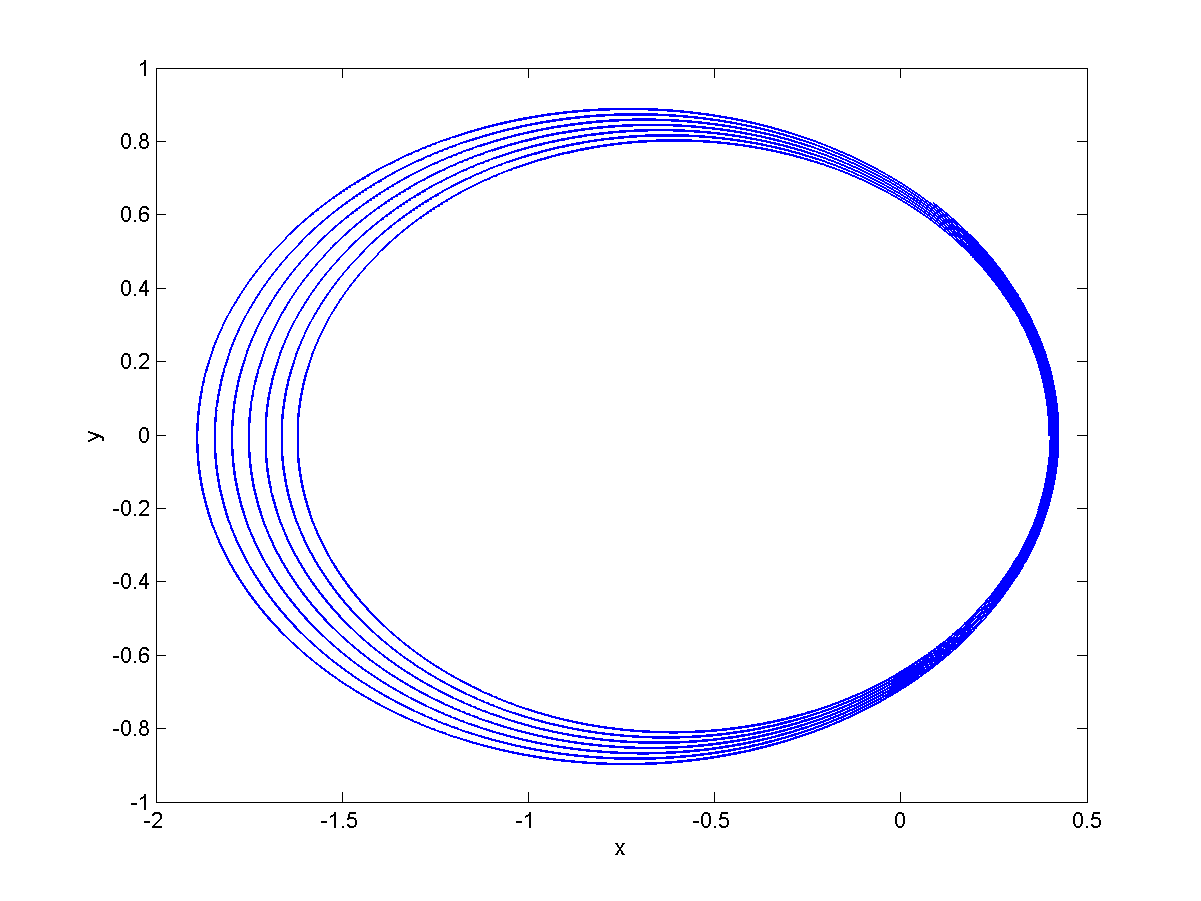
\includegraphics[width=\textwidth]{images/Q1_explicite_q.png}
    \caption{$q$ pour explicite}
    \label{fig:q1_explicite_q}
  \end{subfigure}%
  ~ %add desired spacing between images, e. g. ~, \quad, \qquad etc.
  %(or a blank line to force the subfigure onto a new line)
  \begin{subfigure}[b]{0.45\textwidth}
    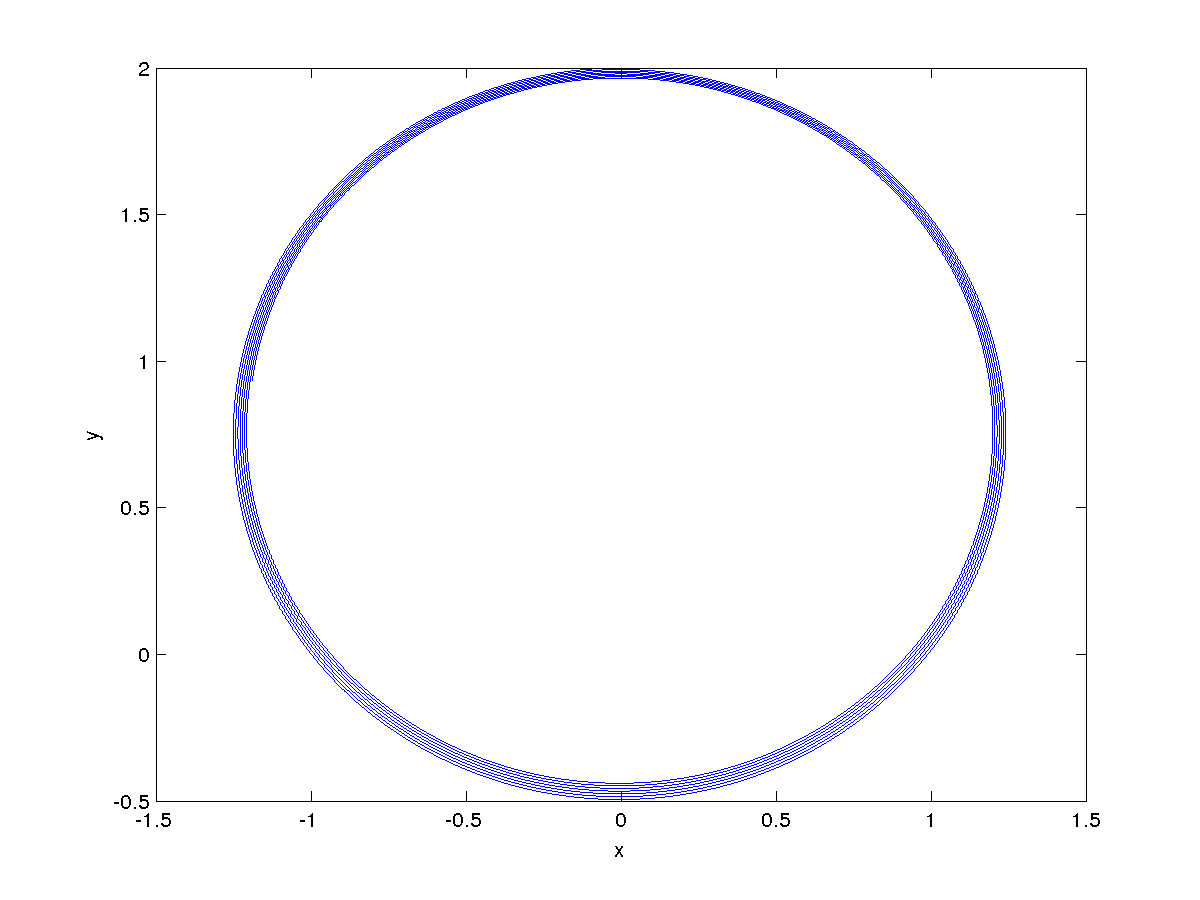
\includegraphics[width=\textwidth]{images/Q1_explicite_p.png}
    \caption{$p$ pour explicite}
    \label{fig:q1_explicite_p}
  \end{subfigure}
  \begin{subfigure}[b]{0.45\textwidth}
    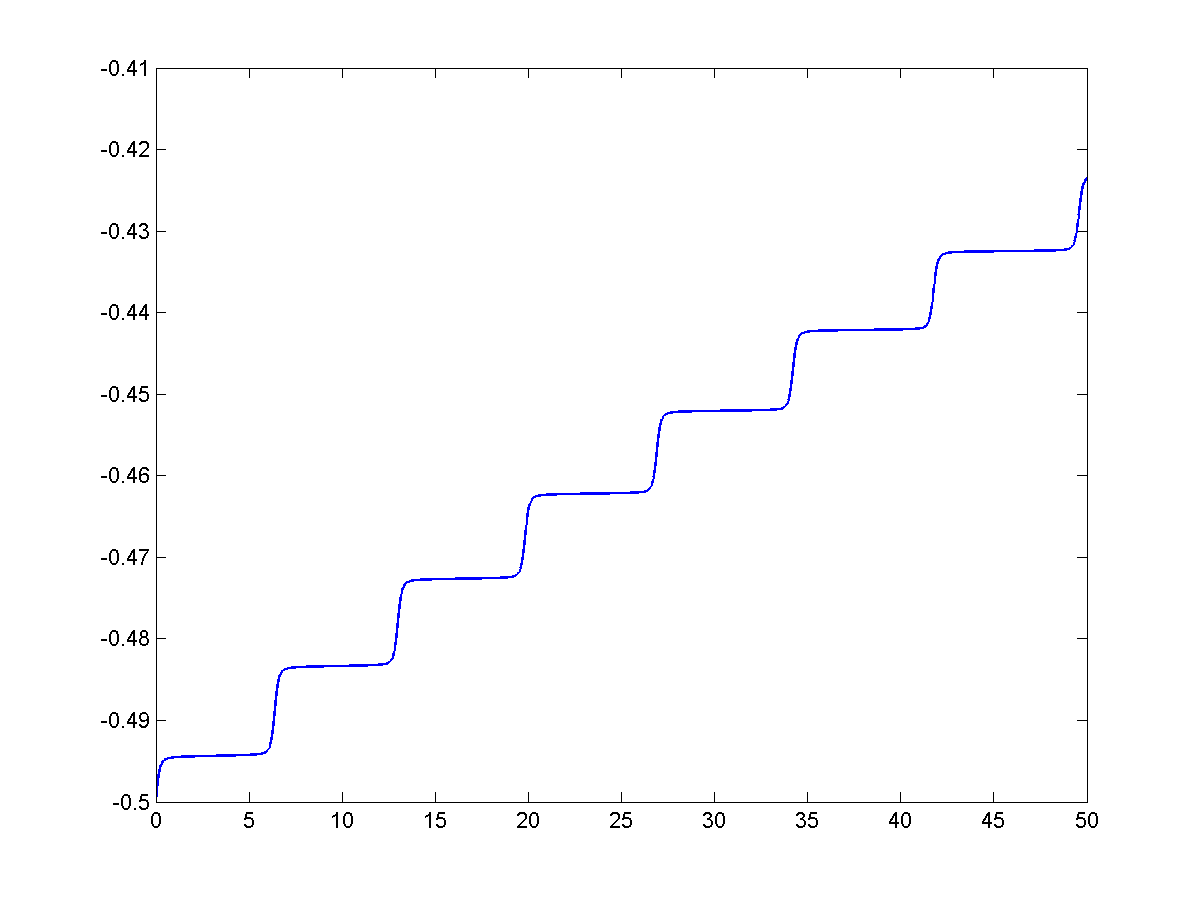
\includegraphics[width=\textwidth]{images/Q1_explicite_H.png}
    \caption{$\Ha$ pour explicite}
    \label{fig:q1_explicite_H}
  \end{subfigure}
  \caption{Résultats pour euler explicite}\label{fig:q1_explicite}
\end{figure}

\begin{figure}
  \centering
  \begin{subfigure}[b]{0.45\textwidth}
    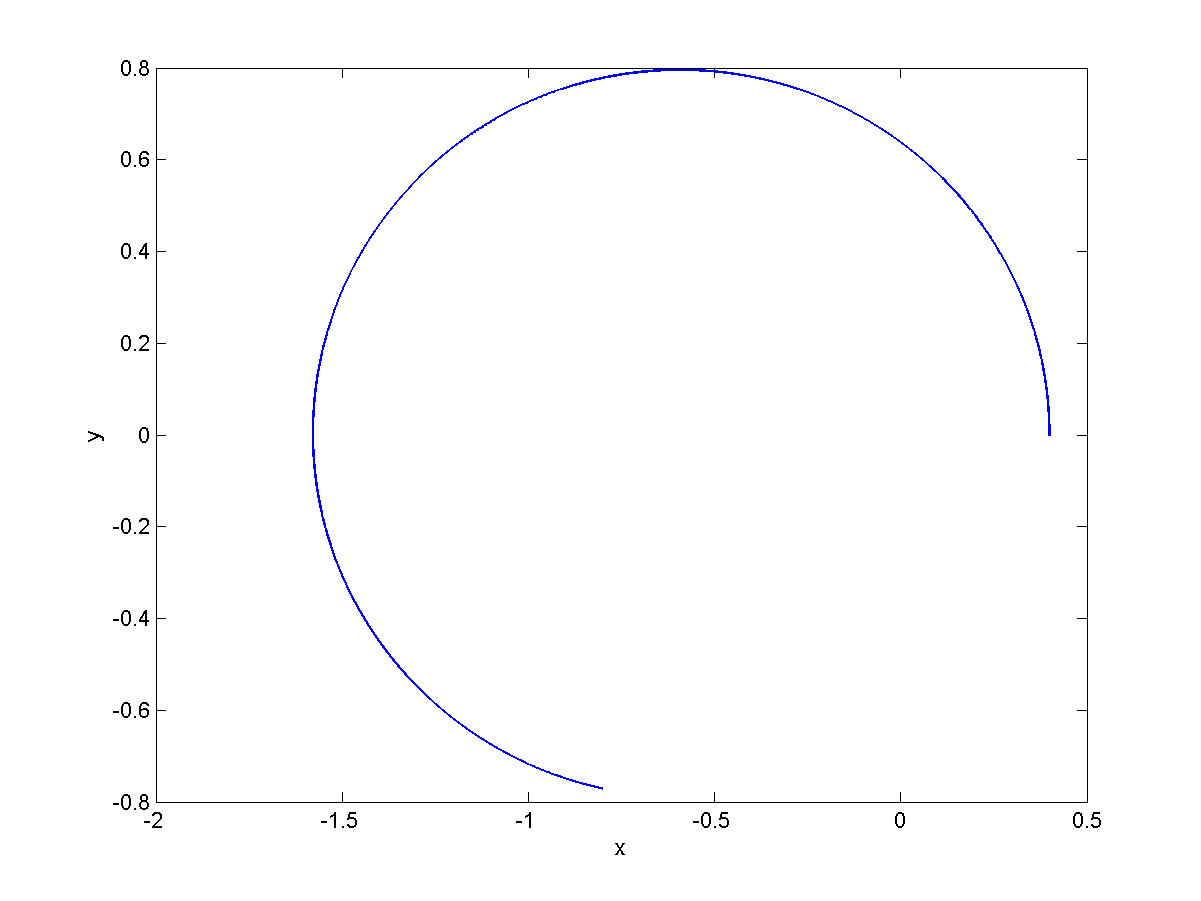
\includegraphics[width=\textwidth]{images/Q1_implicite_q.png}
    \caption{$q$ pour implicite}
    \label{fig:q1_implicite_q}
  \end{subfigure}%
  ~ %add desired spacing between images, e. g. ~, \quad, \qquad etc.
  %(or a blank line to force the subfigure onto a new line)
  \begin{subfigure}[b]{0.45\textwidth}
    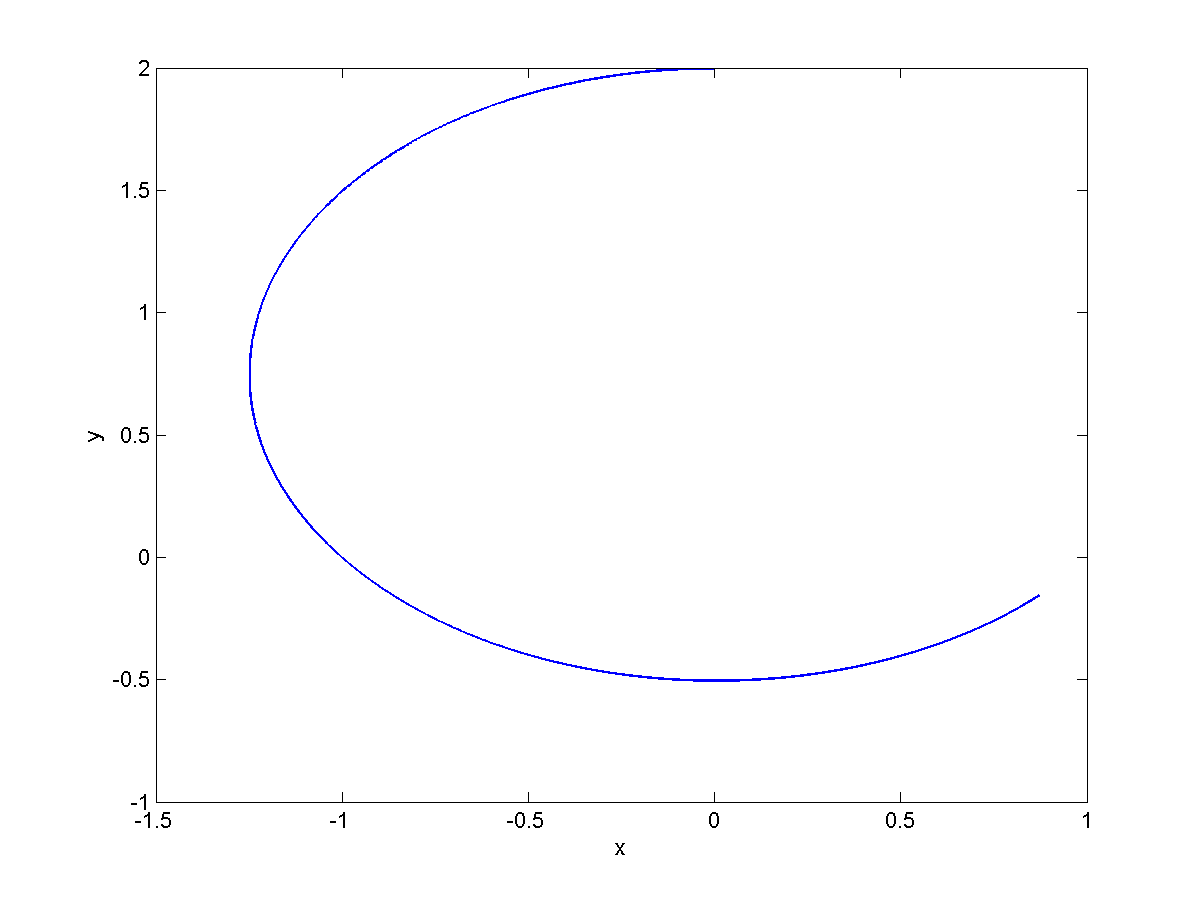
\includegraphics[width=\textwidth]{images/Q1_implicite_p.png}
    \caption{$p$ pour implicite}
    \label{fig:q1_implicite_p}
  \end{subfigure}
  \begin{subfigure}[b]{0.45\textwidth}
    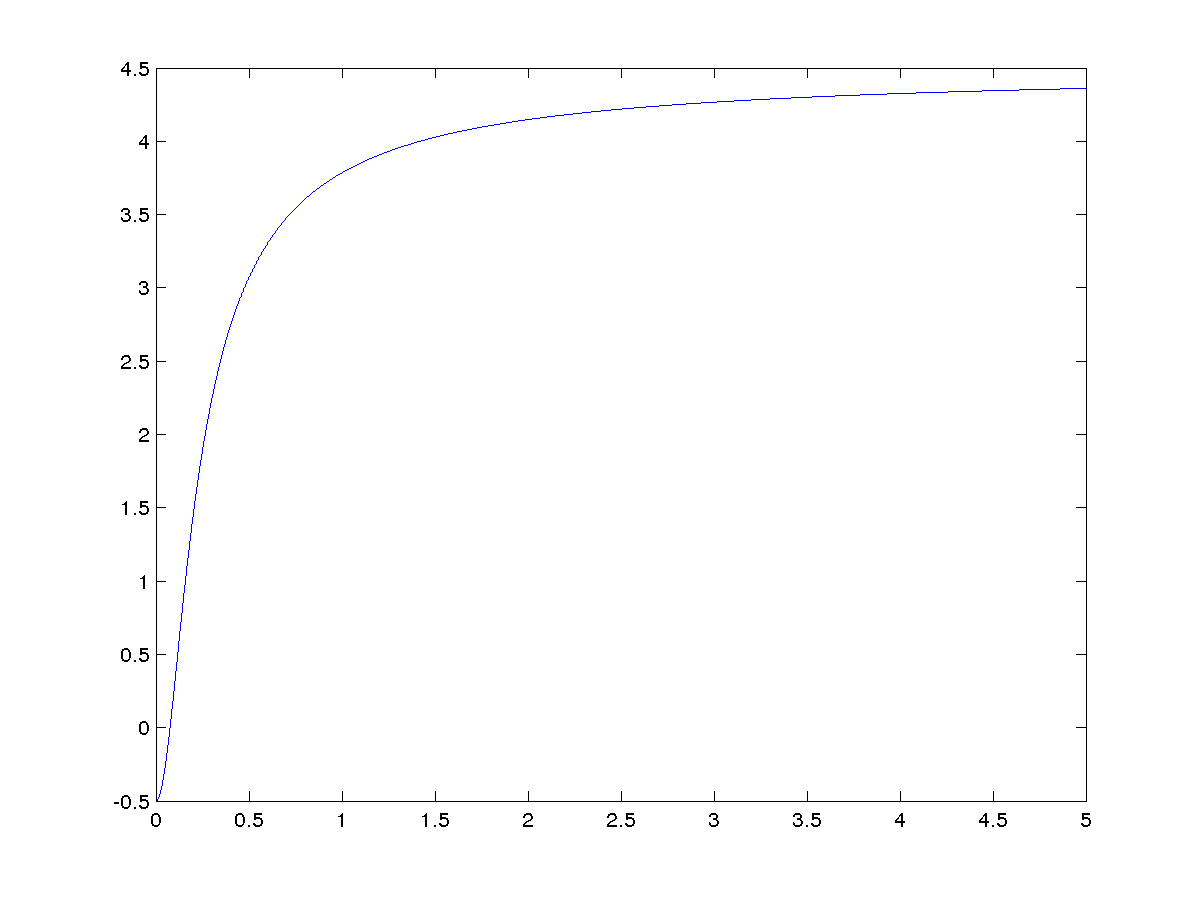
\includegraphics[width=\textwidth]{images/Q1_implicite_H.png}
    \caption{$\Ha$ pour implicite}
    \label{fig:q1_implicite_H}
  \end{subfigure}
  \caption{Résultats pour euler implicite}\label{fig:q1_implicite}
\end{figure}
